\documentclass[tikz,border=10pt]{standalone}
\usepackage[utf8]{inputenc}
\usepackage{tikz}
\usepackage{colortbl}
\usetikzlibrary{shapes,arrows.meta,positioning,calc,fit}

\definecolor{ScoutGreen}{HTML}{005432}
\definecolor{ScoutNavy}{HTML}{002855}
\definecolor{ScoutBlue}{HTML}{006EB6}
\definecolor{ScoutRed}{HTML}{A31920}
\definecolor{BorderGray}{HTML}{CBD5E1}

\begin{document}
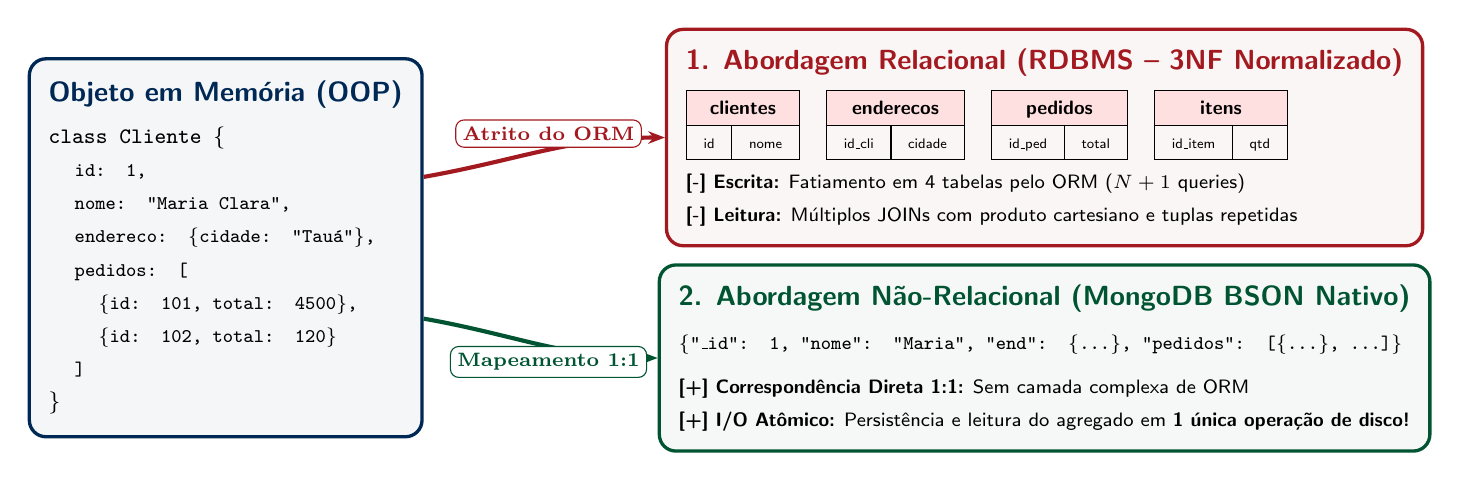
\begin{tikzpicture}[
    font=\sffamily,
    codebox/.style={draw=#1, rounded corners=6pt, fill=#1!4, line width=1.2pt, inner sep=7pt, align=left},
    arrow/.style={-{Stealth[length=6pt]}, line width=1.5pt}
]

  % -------------------------------------------------------------
  % LADO ESQUERDO: DOMÍNIO ORIENTADO A OBJETOS (MEMÓRIA RAM)
  % -------------------------------------------------------------
  \node[codebox=ScoutNavy, minimum width=4.4cm, minimum height=4.8cm] (obj) at (0, 0) {
    \textbf{\textcolor{ScoutNavy}{Objeto em Memória (OOP)}}\\[3pt]
    \footnotesize\texttt{class \textbf{Cliente} \{}\\
    \scriptsize\texttt{\hspace*{2mm} id: 1,}\\
    \scriptsize\texttt{\hspace*{2mm} nome: "Maria Clara",}\\
    \scriptsize\texttt{\hspace*{2mm} endereco: \{cidade: "Tauá"\},}\\
    \scriptsize\texttt{\hspace*{2mm} pedidos: [}\\
    \scriptsize\texttt{\hspace*{5mm} \{id: 101, total: 4500\},}\\
    \scriptsize\texttt{\hspace*{5mm} \{id: 102, total: 120\}}\\
    \scriptsize\texttt{\hspace*{2mm} ]}\\
    \footnotesize\texttt{\}}
  };

  % -------------------------------------------------------------
  % RAMO SUPERIOR: RELACIONAL (FRAGMENTAÇÃO & ORM)
  % -------------------------------------------------------------
  \node[codebox=ScoutRed, minimum width=8.8cm] (rdbms) at (10.4, 1.4) {
    \textbf{\textcolor{ScoutRed}{1. Abordagem Relacional (RDBMS -- 3NF Normalizado)}}\\[4pt]
    \begin{tabular}{|l|l|}
      \hline
      \multicolumn{2}{|c|}{\cellcolor{red!12}\scriptsize\textbf{clientes}} \\
      \hline
      \tiny id & \tiny nome \\
      \hline
    \end{tabular}
    \hspace{1mm}
    \begin{tabular}{|l|l|}
      \hline
      \multicolumn{2}{|c|}{\cellcolor{red!12}\scriptsize\textbf{enderecos}} \\
      \hline
      \tiny id\_cli & \tiny cidade \\
      \hline
    \end{tabular}
    \hspace{1mm}
    \begin{tabular}{|l|l|}
      \hline
      \multicolumn{2}{|c|}{\cellcolor{red!12}\scriptsize\textbf{pedidos}} \\
      \hline
      \tiny id\_ped & \tiny total \\
      \hline
    \end{tabular}
    \hspace{1mm}
    \begin{tabular}{|l|l|}
      \hline
      \multicolumn{2}{|c|}{\cellcolor{red!12}\scriptsize\textbf{itens}} \\
      \hline
      \tiny id\_item & \tiny qtd \\
      \hline
    \end{tabular}\\[4pt]
    \scriptsize \textbf{[-] Escrita:} Fatiamento em 4 tabelas pelo ORM ($N+1$ queries)\\
    \scriptsize \textbf{[-] Leitura:} Múltiplos JOINs com produto cartesiano e tuplas repetidas
  };

  % Seta para Relacional com badge explicitamente centrado
  \draw[arrow, color=ScoutRed] ($(obj.east)+(0, 0.9)$) to[out=10, in=180] (rdbms.west);
  \node[fill=white, draw=ScoutRed, rounded corners=3pt, font=\scriptsize\bfseries, text=ScoutRed, inner sep=2.5pt] at (4.1, 1.45) {Atrito do ORM};

  % -------------------------------------------------------------
  % RAMO INFERIOR: NOSQL DOCUMENTOS (AGREGADO BSON 1:1)
  % -------------------------------------------------------------
  \node[codebox=ScoutGreen, minimum width=8.8cm] (nosql) at (10.4, -1.4) {
    \textbf{\textcolor{ScoutGreen}{2. Abordagem Não-Relacional (MongoDB BSON Nativo)}}\\[4pt]
    \scriptsize\texttt{\{"\_id": 1, "nome": "Maria", "end": \{...\}, "pedidos": [\{...\}, ...]\}}\\[4pt]
    \scriptsize \textbf{[+] Correspondência Direta 1:1:} Sem camada complexa de ORM\\
    \scriptsize \textbf{[+] I/O Atômico:} Persistência e leitura do agregado em \textbf{1 única operação de disco!}
  };

  % Seta para NoSQL com badge explicitamente centrado
  \draw[arrow, color=ScoutGreen] ($(obj.east)+(0, -0.9)$) to[out=-10, in=180] (nosql.west);
  \node[fill=white, draw=ScoutGreen, rounded corners=3pt, font=\scriptsize\bfseries, text=ScoutGreen, inner sep=2.5pt] at (4.1, -1.45) {Mapeamento 1:1};

\end{tikzpicture}
\end{document}
